\section{Motivation}
\label{flexheap:sec:motiv}

We motivate the need for a dynamic heap-resizing mechanism that accounts for both \flexheapGC{} and I/O stalls.
Specifically, we show that existing heap-resizing mechanisms fail to adapt to the phase behavior of applications, whose heap and I/O cache demands vary over time.
To illustrate this limitation, we use Elasticsearch, a widely used production-grade search engine deployed at scale for log analytics, full-text search, and observability workloads.
We run the Wikipedia workload that performs concurrently search and document ingestion.
During ingestion, incoming documents are indexed and made searchable.
Section~\S~\ref{flexheap:sec:methodology} describes the full experimental setup.

\begin{figure*}[t]
	
\includegraphics[width=0.6\linewidth]{flexheap/fig/motiv/legend.pdf}
	\\
	\subfloat[G1-90]{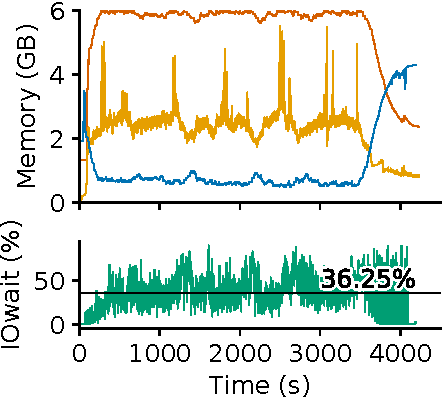
\includegraphics[width=0.245\linewidth]{flexheap/fig/motiv/nat90_ci4_cs32_d8g.pdf}}
	\subfloat[G1-50]{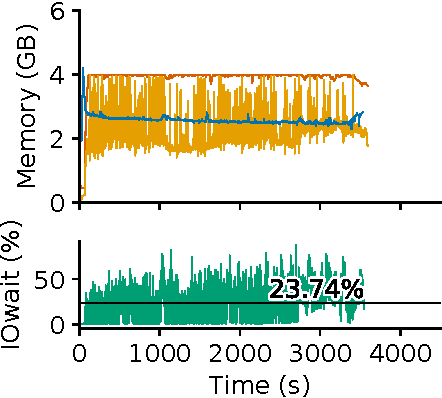
\includegraphics[width=0.245\linewidth]{flexheap/fig/motiv/nat50_ci4_cs32_d8g.pdf}}
	\subfloat[VG1]{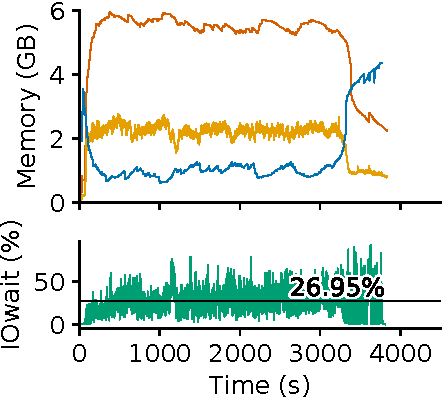
\includegraphics[width=0.245\linewidth]{flexheap/fig/motiv/je_ci4_cs32_d8g.pdf}}
	\subfloat[\flexheapName{}]{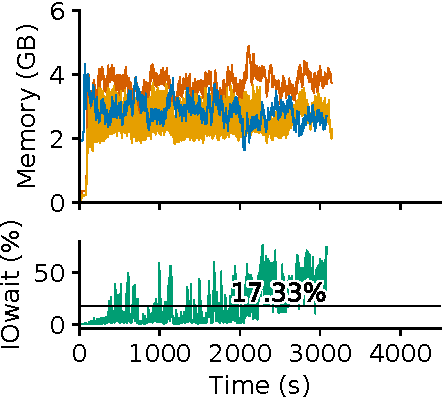
\includegraphics[width=0.245\linewidth]{flexheap/fig/motiv/fh_ci4_cs32_d8g.pdf}}
	\caption{
		Heap usage, I/O cache occupancy, and I/O wait over time for the Wikipedia workload in Elasticsearch:
		(a) G1-90 (with a maximum heap cap of 90\% of DRAM),
		(b) G1-50 (with a maximum heap cap of 50\% of DRAM),
		(c) VG1, and
		(d) \flexheapName{}.
	}
	\label{flexheap:fig:motiv}
\end{figure*}

\begin{figure}[t]
	
\includegraphics[width=0.4\linewidth]{flexheap/fig/motiv/xput_legend.pdf}
	\\
	\subfloat[Throughput]{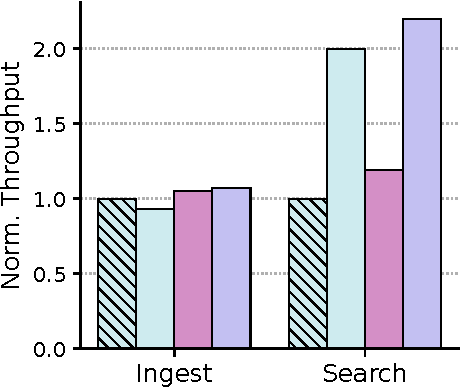
\includegraphics[width=0.3\linewidth]{flexheap/fig/motiv/xput.pdf}}
	\hspace{10pt}
	\subfloat[Latency]{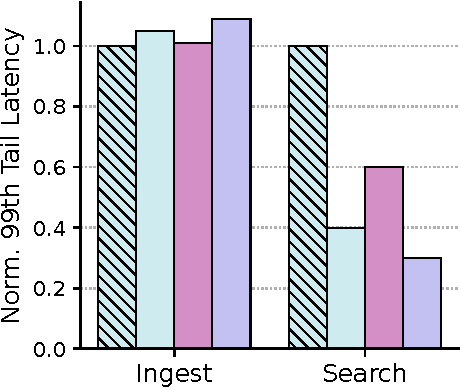
\includegraphics[width=0.3\linewidth]{flexheap/fig/motiv/lat.pdf}}
	\caption{Normalized document ingestion and query search (a) throughput, and
		(b) p99 latency for the Wikipedia workload in Elasticsearch under G1-90
		(with a maximum heap cap of 90\% of DRAM), G1-50 (with a maximum heap cap
		of 50\% of DRAM), VG1, and \flexheapName{}. Results are normalized to G1-90.}
	\label{fig:motiv:xput_lat}
\end{figure}

\subsection{GC-Based Heap Resizing Mechanisms Prioritize the Heap Over the I/O Cache}
\label{sec:gc_driven}

G1’s heap resizing mechanism cannot adapt to workloads that simultaneously stress the heap and the I/O cache because it relies solely on GC metrics.
In Figure~\ref{flexheap:fig:motiv}(a), we use G1 with the heap capped at 90\% of the available system DRAM (G1-90) on Elasticsearch running the Wikipedia workload.
Document ingestion and search run in parallel from the start until about \SI{3500}{s}, after which only search continues.
During this mixed phase, G1 continues to expand the committed heap until it reaches the configured cap.
Because its decisions consider only GC cost, G1 assigns nearly all available DRAM to the heap, leaving little space for the I/O cache; as a result, I/O wait remains high (about 36\% on average) for most of the execution.
After ingestion ends, heap usage drops to approximately \SI{1}{GB}, and the collector gradually returns memory to the OS; therefore, shrinking occurs only once heap pressure subsides.

Following Elasticsearch guidelines~\cite{elasticsearch:guidelines}, we cap the heap at 50\% of DRAM (G1-50) and run the same workload.
G1’s dynamic resizing remains active but is constrained by this cap.
Using G1-50, the execution time decreases by 15\% compared to G1-90.
This improvement is mainly due to the reduction of the average I/O wait by 24\% (a 33\% improvement over G1-90) because the I/O cache remains larger (approximately \SI{3}{GB}).
However, the cap restricts heap growth during document ingestion and consequently drives up GC activity: 54 full GCs instead of 1 in G1-90, plus 2{,}530 additional young and mixed GCs overall.
Under G1-50, document ingestion tasks run until the end of execution, resulting in 8\% lower document ingestion throughput compared to G1-90 (Figure~\ref{fig:motiv:xput_lat}(a)).
Conversely, the consistently larger I/O cache under G1-50 improves query performance: Figure~\ref{fig:motiv:xput_lat}(a) shows that search throughput is $2\times$ higher than under G1-90, and Figure~\ref{fig:motiv:xput_lat}(b) shows that p99 latency is 62\% lower.
This improvement primarily stems from a $2.4\times$ reduction in device read traffic compared to G1-90.

\subsection{Occupancy-Based Heap Resizing Mechanisms Ignore I/O Cost}
\label{sec:occupancy_driven}

Next, we examine whether time-driven, occupancy-based mechanisms, such as VG1, that return memory to the OS more aggressively can reduce I/O overhead.
As shown in Figure~\ref{flexheap:fig:motiv}(c), VG1 improves execution time by 5\% upon G1-90 but is insufficient without I/O awareness: during mixed phases, the heap remains near the cap and the I/O cache is constrained.
VG1 improves performance relative to G1-90 by reducing average I/O wait from 36\% to 27\% and increasing document ingestion throughput by 5\%.
However, it remains inferior compared to G1-50.
As VG1 does not adapt within the mixed ingestion–search phase, it continues to allocate most DRAM to the heap rather than the I/O cache when needed.
Consequently, Figure~\ref{fig:motiv:xput_lat}(a) shows that search throughput is approximately 40\% lower than G1-50, which maintains a larger I/O cache by capping the heap at 50\% of DRAM (at the cost of increased GC activity and lower document ingestion throughput).

\subsection{Considering Both GC and I/O Costs for Heap Resizing}

Figure~\ref{flexheap:fig:motiv}(d) shows \flexheapName{}, which resizes the heap using both \flexheapGC{} and I/O feedback.
During the mixed phase, it prevents the heap from monopolizing DRAM, leaving sufficient room for the I/O cache.
These results indicate that considering both \flexheapGC{} and I/O stalls enables more efficient DRAM use and higher end-to-end performance.
We present detailed results in the Section~\S\ref{flexheap:sec:eval}.
